\documentclass[12pt]{article}

%\usepackage{brain_damage}

\usepackage{graphicx}
\usepackage{a4wide}

\def\MAGIC{MAGIC}

\begin{document}

\title{William Wilson}
\author{E. A. Poe}
\date{}

\maketitle

\hfill
\parbox[b]{8cm}{
\scriptsize
What say of it? what say of CONSCIENCE grim,\\
That spectre in my path?\\
\mbox{}\hspace{2cm} \scshape{Chamberlayne}'s \emph{Pharronida}\\
}

\vskip 1cm

     Let me call myself, for the present, William Wilson.  The fair
page now lying before me need not be sullied with my real
appellation.  This has been already too much an object for the
scorn--for the horror--for the detestation of my race.  To the
uttermost regions of the globe have not the indignant winds bruited
its unparalleled infamy?  Oh, outcast of all outcasts most
abandoned!--to the earth art thou not forever dead? to its honours,
to its flowers, to its golden aspirations?--and a cloud, dense,
dismal, and limitless, does it not hang eternally between thy hopes
and heaven?

     I would not, if I could, here or to-day, embody a record of my
later years of unspeakable misery, and unpardonable crime.  This
epoch--these later years--took unto themselves a sudden elevation
in turpitude, whose origin alone it is my present purpose to
assign.  Men usually grow base by degrees.  From me, in an instant,
all virtue dropped bodily as a mantle.  From comparatively trivial
wickedness I passed, with the stride of a giant, into more than the
enormities of an Elah-Gabalus.  What a chance--what one event
brought this evil thing to pass, bear with me while I relate. 
Death approaches; and the shadow which foreruns him has thrown a
softening influence over my spirit.  I long, in passing through the
dim valley, for the sympathy--I had nearly said for the pity--of my
fellow-men.  I would fain have them believe that I have been, in
some measure, the slave of circumstances beyond human control.  I
would wish them to seek out for me, in the details I am about to
give, some little oasis of \emph{fatality} amid a wilderness of error. 
I would have them allow--what they cannot refrain from allowing--
that, although temptation may have erewhile existed as great, man
was never \emph{thus}, at least, tempted before--certainly, never 
\emph{thus} fell.  And is it therefore that he has never thus suffered? 
Have I not indeed been living in a dream?  And am I not now dying
a victim to the horror and the mystery of the wildest of all
sublunary visions?  

     I am the descendant of a race whose imaginative and easily
excitable temperament has at all times rendered them remarkable;
and, in my earliest infancy, I gave evidence of having fully
inherited the family character.  As I advanced in years it was more
strongly developed; becoming, for many reasons, a cause of serious
disquietude to my friends, and of positive injury to myself.  I
grew self-willed, addicted to the wildest caprices, and a prey to
the most ungovernable passions.  Weak-minded, and beset with
constitutional infirmities akin to my own, my parents could do but
little to check the evil propensities which distinguished me.  Some
feeble and ill-directed efforts resulted in complete failure on
their part, and, of course, in total triumph on mine. 
Thenceforward my voice was a household law; and at an age when few
children have abandoned their leading-strings, I was left to the
guidance of my own will, and became, in all but name, the master of
my own actions.

     My earliest recollections of a school-life, are connected with
a large, rambling, Elizabethan house, in a misty-looking village of
England, where were a vast number of gigantic and gnarled trees,
and where all the houses were excessively ancient.  In truth, it
was a dream-like and spirit-soothing place, that venerable old
town.  At this moment, in fancy, I feel the refreshing chilliness
of its deeply-shadowed avenues, inhale the fragrance of its
thousand shrubberies, and thrill anew with undefinable delight, at
the deep hollow note of the church-bell, breaking, each hour, with
sullen and sudden roar, upon the stillness of the dusky atmosphere
in which the fretted Gothic steeple lay imbedded and asleep.

     It gives me, perhaps, as much of pleasure as I can now in any
manner experience, to dwell upon minute recollections of the school
and its concerns.  Steeped in misery as I am--misery, alas! only
too real--I shall be pardoned for seeking relief, however slight
and temporary, in the weakness of a few rambling details.  These,
moreover, utterly trivial, and even ridiculous in themselves,
assume, to my fancy, adventitious importance, as connected with a
period and a locality when and where I recognize the first
ambiguous monitions of the destiny which afterwards so fully
overshadowed me.  Let me then remember.

     The house, I have said, was old and irregular.  The grounds
were extensive, and a high and solid brick wall, topped with
a bed of mortar and broken glass, encompassed the whole.  This
prison-like rampart formed the limit of our domain; beyond it we
saw but thrice a week--once every Saturday afternoon, when,
attended by two ushers, we were permitted to take brief walks in a
body through some of the neighbouring fields--and twice during
Sunday, when we were paraded in the same formal manner to the
morning and evening service in the one church of the village.  Of
this church the principal of our school was pastor.  With how deep
a spirit of wonder and perplexity was I wont to regard him from our
remote pew in the gallery, as, with step solemn and slow, he
ascended the pulpit!  This reverend man, with countenance so
demurely benign, with robes so glossy and so clerically flowing,
with wig so minutely powdered, so rigid and so vast,--could this be
he who, of late, with sour visage, and in snuffy habiliments,
administered, ferule in hand, the Draconian laws of the academy? 
Oh, gigantic paradox, too utterly monstrous for solution!

     At an angle of the ponderous wall frowned a more ponderous
gate.  It was riveted and studded with iron bolts, and surmounted
with jagged iron spikes.  What impression of deep awe did it
inspire!  It was never opened save for the three periodical
egressions and ingressions already mentioned; then, in every creak
of its mighty hinges, we found a plenitude of mystery--a world of
matter for solemn remark, or for more solemn meditation.

     The extensive enclosure was irregular in form, having many
capacious recesses.  Of these, three or four of the largest
constituted the play-ground.  It was level, and covered with fine
hard gravel.  I well remember it had no trees, nor benches, nor
anything similar within it.  Of course it was in the rear of the
house.  In front lay a small parterre, planted with box and other
shrubs; but through this sacred division we passed only upon rare
occasions indeed--such as a first advent to school or final
departure thence, or perhaps, when a parent or friend having called
for us, we joyfully took our way home for the Christmas or
Midsummer holidays.

     But the house!--how quaint an old building was this!--to me
how veritably a place of enchantment!  There was really no end to
its windings--to its incomprehensible subdivisions.  It was
difficult at any given time, to say with certainty upon which of
its two stories one happened to be.  From each room to every
other there were sure to be found three or four steps either in
ascent or descent.  Then the lateral branches were innumerable--
inconceivable--and so returning in upon themselves, that our most
exact ideas in regard to the whole mansion were not very far
different from those with which we pondered upon infinity.  During
the five years of my residence here, I was never able to ascertain
with precision, in what remote locality lay the little sleeping
apartment assigned to myself and some eighteen or twenty other
scholars.

     The school-room was the largest in the house--I could not help
thinking, in the world.  It was very long, narrow, and dismally
low, with pointed Gothic windows and a ceiling of oak.  In a remote
and terror-inspiring angle was a square enclosure of eight or ten
feet, comprising the \emph{sanctum}, 'during hours', or our principal,
the Reverend Dr Bransby.  It was a solid structure, with massy
door, sooner than open which in the absence of the 'Dominie', we
would all have willingly perished by the \emph{peine forte et dure}. 
In other angles were two other similar boxes, far less reverenced,
indeed, but still greatly matters of awe.  One of these was the
pulpit of the 'classical' usher, one of the 'English and
mathematical'.  Interspersed about the room, crossing and
recrossing in endless irregularity, were innumerable benches and
desks, black, ancient, and time-worn, piled desperately with much-
bethumbed books, and so beseamed with initial letters, names at
full length, grotesque figures, and other multiplied efforts of the
knife, as to have entirely lost what little of original form might
have been their portion in days long departed.  A huge bucket with
water stood at one extremity of the room, and a clock of stupendous
dimensions at the other.

     Encompassed by the massy walls of this venerable academy, I
passed, yet not in tedium or disgust, the years of the third
lustrum of my life.  The teeming brain of childhood requires no
external world of incident to occupy or amuse it; and the
apparently dismal monotony of a school was replete with more
intense excitement than my riper youth has derived from luxury, or
my full manhood from crime.  Yet I must believe that my first
mental development had in it much of the uncommon--even much of the
\emph{outre}.  Upon mankind at large the events of very early
existence rarely leave in mature age any definite impression. 
All is grey shadow--a weak and irregular remembrance--an indistinct
regathering of feeble pleasures and phantasmagoric pains.  With me
this is not so.  In childhood I must have felt with the energy of
a man what I now find stamped upon memory in lines as vivid, as
deep, and as durable as the \emph{exergues} of the Carthaginian
medals.

     Yet in fact--in the fact of the world's view--how little was
there to remember!  The morning's awakening, the nightly summons to
bed; the connings, the recitations; the periodical half-holidays,
and perambulations; the play-ground, with its broils, its pastimes,
its intrigues;--these, by a mental sorcery long forgotten, were
made to involve a wilderness of sensation, a world of rich
incident, a universe of varied emotion, of excitement the most
passionate and spirit-stirring.  '\emph{Oh, le bon temps, que ce
siecle de fer}!'

     In truth, the ardour, the enthusiasm, and the imperiousness of
my disposition, soon rendered me a marked character among my
schoolmates, and by slow, but natural gradations, gave me an
ascendancy over all not greatly older than myself;--over all with
a single exception.  This exception was found in the person of a
scholar, who, although no relation, bore the same Christian and
surname as myself;--a circumstance, in fact, little remarkable;
for, notwithstanding a noble descent, mine was one of those every-
day appellations which seem, by prescriptive right, to have been,
time out of mind, the common property of the mob.  In this
narrative I have therefore designated myself as William Wilson,--a
fictitious title not very dissimilar to the real.  My namesake
alone, of those who in school phraseology constituted 'our set',
presumed to compete with me in the studies of the class--in the
sports and broils of the play-ground--to refuse implicit belief in
my assertions, and submission to my will--indeed, to interfere with
my arbitrary dictation in any respect whatsoever.  If there is on
earth a supreme and unqualified despotism, it is the despotism of
a master mind in boyhood over the less energetic spirits of its
companions.

     Wilson's rebellion was to me a source of the greatest
embarrassment;--the more so as, in spite of the bravado with which
in public I made a point of treating him and his pretensions, I
secretly felt that I feared him, and could not help thinking the
equality which he maintained so easily with myself, a proof
of his true superiority; since not to be overcome cost me a
perpetual struggle.  Yet this superiority--even this equality--was
in truth acknowledged by no one but myself; our associates, by some
unaccountable blindness, seemed not even to suspect it.  Indeed,
his competition, his resistance, and especially his impertinent and
dogged interference with my purposes, were not more pointed than
private.  He appeared to be destitute alike of the ambition which
urged, and of the passionate energy of mind which enabled me to
excel.  In his rivalry he might have been supposed actuated solely
by a whimsical desire to thwart, astonish, or mortify myself;
although there were times when I could not help observing, with a
feeling made up of wonder, abasement, and pique, that he mingled
with his injuries, his insults, or his contradictions, a certain
most inappropriate, and assuredly most unwelcome 
\emph{affectionateness} of manner.  I could only conceive this singular
behaviour to arise from a consummate self-conceit assuming the
vulgar air of patronage and protection.

     Perhaps it was this latter trait in Wilson's conduct,
conjoined with our identity of name, and the mere accident of our
having entered the school upon the same day, which set afloat the
notion that we were brothers, among the senior classes in the
academy.  These do not usually inquire with much strictness into
the affairs of their juniors.  I have before said, or should have
said, that Wilson was not, in the most remote degree, connected
with my family.  But assuredly if we \emph{had} been brothers we must
have been twins; for, after leaving Dr Bransby's, I casually
learned that my namesake was born on the nineteenth of January,
1813--and this is a somewhat remarkable coincidence; for the day is
precisely that of my own nativity.

     It may seem strange that in spite of the continual anxiety
occasioned me by the rivalry of Wilson, and his intolerable spirit
of contradiction, I could not bring myself to hate him altogether. 
We had, to be sure, nearly every day a quarrel in which, yielding
me publicly the palm of victory, he, in some manner, contrived to
make me feel that it was he who had deserved it; yet a sense of
pride on my part, and a veritable dignity on his own, kept us
always upon what are called 'speaking terms', where there were 
 many points of strong congeniality in our tempers, operating to
awake in me a sentiment which our position alone, perhaps,
prevented from ripening into friendship.  It is difficult, indeed,
to define, or even to describe, my real feelings towards him.  They
formed a motley and heterogeneous admixture;--some petulant
animosity, which was not yet hatred, some esteem, more respect,
much fear, with a world of uneasy curiosity.  To the moralist it
will be unnecessary to say, in addition, that Wilson and myself
were the most inseparable of companions.

     It was no doubt the anomalous state of affairs existing
between us, which turned all my attacks upon him (and they were
many, either open or covert) into the channel of banter or
practical joke (giving pain while assuming the aspect of mere fun)
rather than into a more serious and determined hostility.  But my
endeavours on this head were by no means uniformly successful, even
when my plans were the most wittily concocted; for my namesake had
much about him, in character, of that unassuming and quiet
austerity which, while enjoying the poignancy of its own jokes, has
no heel of Achilles in itself, and absolutely refuses to be laughed
at.  I could find, indeed, but one vulnerable point, and that,
lying in a personal peculiarity, arising, perhaps, from
constitutional disease, would have been spared by any antagonist
less at his wit's end than myself--my rival had a weakness in the
faucial or guttural organs, which precluded him from raising his
voice at any time \emph{above a very low whisper}.  Of this defect I
did not fail to take what poor advantage lay in my power.

     Wilson's retaliations in kind were many; and there was one
form of his practical wit that disturbed me beyond measure.  How
his sagacity first discovered at all that so petty a thing would
vex me, is a question I never could solve; but, having discovered,
he habitually practised the annoyance.  I had always felt aversion
to my uncourtly patronymic, and its very common, if not plebeian
praenomen.  The words were venom in my ears; and when, upon the day
of my arrival, a second William Wilson came also to the academy, I
felt angry with him for bearing the name, and doubly disgusted with
the name because a stranger bore it, who would be the cause of its
two-fold repetition, who would be constantly in my presence, and
whose concerns, in the ordinary routine of the  school
business, must inevitably, on account of the detestable
coincidence, be often confounded with my own.

     The feeling of vexation thus engendered grew stronger with
every circumstance tending to show resemblance, moral or physical,
between my rival and myself.  I had not then discovered the
remarkable fact that we were of the same age; but I saw that we
were of the same height, and I perceived that we were even
singularly alike in general contour of person and outline of
feature.  I was galled, too, by the rumour touching a relationship,
which had grown current in the upper forms.  In a word, nothing
could more seriously disturb me (although I scrupulously concealed
such disturbance), than any allusion to a similarity of mind,
person, or condition existing between us.  But, in truth, I had no
reason to believe that (with the exception of the matter of
relationship, and in the case of Wilson himself) this similarity
had ever been made a subject of comment, or even observed at all by
our schoolfellows.  That \emph{he} observed it in all its bearings,
and as fixedly as I, was apparent; but that he could discover in
such circumstances so fruitful a field of annoyance, can only be
attributed, as I said before, to his more than usual penetration.

     His cue, which was to perfect an imitation of myself, lay both
in words and in actions; and most admirably did he play his part. 
My dress it was an easy matter to copy; my gait and general manner
were, without difficulty, appropriated; in spite of his
constitutional defect, even my voice did not escape him.  My louder
tones were, of course, unattempted, but then the key, it was
identical; \emph{and his singular whisper, it grew the very echo of my
own}.

     How greatly this most exquisite portraiture harassed me (for
it could not justly be termed a caricature), I will not now venture
to describe.  I had but one consolation--in the fact that the
imitation, apparently, was noticed by myself alone, and that I had
to endure only the knowing and strangely sarcastic smiles of my
namesake himself.  Satisfied with having produced in my bosom the
intended effect, he seemed to chuckle in secret over the sting he
had inflicted, and was characteristically disregardful of the
public applause which the success of his witty endeavours might
have so easily elicited.  That the school, indeed, did not feel his
design, perceive its accomplishment, and participate in his
sneer, was, for many anxious months, a riddle I could not resolve. 
Perhaps the \emph{gradation} of his copy rendered it not so readily
perceptible; or, more possibly, I owed my security to the masterly
air of the copyist, who, disdaining the letter (which in a painting
is all the obtuse can see), gave but the full spirit of his
original for my individual contemplation and chagrin.

     I have already more than once spoken of the disgusting air of
patronage which he assumed toward me, and of his frequent officious
interference with my will.  This interference often took the
ungracious character of advice; advice not openly given, but hinted
or insinuated.  I received it with a repugnance which gained
strength as I grew in years.  Yet, at this distant day, let me do
him the simple justice to acknowledge that I can recall no occasion
when the suggestions of my rival were on the side of those errors
or follies so usual to his immature age and seeming inexperience;
that his moral sense, at least, if not his general talents and
worldly wisdom, was far keener than my own; and that I might, to-
day, have been a better, and thus a happier man, had I less
frequently rejected the counsels embodied in those meaning whispers
which I then but too cordially hated and too bitterly despised.

     As it was, I at length grew restive in the extreme under his
distasteful supervision, and daily resented more and more openly
what I considered his intolerable arrogance.  I have said that, in
the first years of our connection as schoolmates, my feelings in
regard to him might have been easily ripened into friendship: but,
in the latter months of my residence at the academy, although the
intrusion of his ordinary manner had, beyond doubt, in some
measure, abated, my sentiments, in nearly similar proportion,
partook very much of positive hatred.  Upon one occasion he saw
this, I think, and afterwards avoided, or made a show of avoiding
me.

     It was about the same period, if I remember aright, that, in
an altercation of violence with him, in which he was more than
usually thrown off his guard, and spoke and acted with an openness
of demeanour rather foreign to his nature, I discovered, or fancied
I discovered, in his accent, his air, and general appearance, a
something which first startled, and then deeply interested me, by
bringing to mind dim visions of my earliest infancy--wild, 
confused, and thronging memories of a time when memory herself was
yet unborn.  I cannot better describe the sensation which oppressed
me than by saying that I could with difficulty shake off the belief
of my having been acquainted with the being who stood before me, at
some epoch very long ago--some point of the past even infinitely
remote.  The delusion, however, faded rapidly as it came; and I
mention it at all but to define the day of the last conversation I
there held with my singular namesake.

     The huge old house, with its countless subdivisions, had
several large chambers communicating with each other, where slept
the greater number of the students.  There were, however (as must
necessarily happen in a building so awkwardly planned), many little
nooks or recesses, the odds and ends of the structure; and these
the economic ingenuity of Dr Bransby had also fitted up as
dormitories; although, being the merest closets, they were capable
of accommodating but a single individual.  One of these small
apartments was occupied by Wilson.

     One night, about the close of my fifth year at the school, and
immediately after the altercation just mentioned, finding every one
wrapped in sleep, I arose from bed, and, lamp in hand, stole
through a wilderness of narrow passages from my own bedroom to that
of my rival.  I had long been plotting one of those ill-natured
pieces of practical wit at his expense in which I had hitherto been
so uniformly unsuccessful.  It was my intention, now, to put my
scheme in operation, and I resolved to make him feel the whole
extent of the malice with which I was imbued.  Having reached his
closet, I noiselessly entered, leaving the lamp, with a shade over
it, on the outside.  I advanced a step, and listened to the sound
of his tranquil breathing.  Assured of his being sleep, I returned,
took the light, and with it again approached the bed.  Close
curtains were around it, which, in the prosecution of my plan, I
slowly and quietly withdrew, when the bright rays fell vividly upon
the sleeper, and my eyes, at the same moment, upon his countenance. 
I looked;--and a numbness, an iciness of feeling instantly pervaded
my frame.  My breast heaved, my knees tottered, my whole spirit
became possessed with an objectless yet intolerable horror. 
Gasping for breath, I lowered the lamp in still nearer proximity to
the face.  Were these--\emph{these} the lineaments of  William
Wilson?  I saw, indeed, that they were his, but I shook as if with
a fit of the ague in fancying they were not.  What \emph{was} there
about them to confound me in this manner?  I gazed;--while my brain
reeled with a multitude of incoherent thoughts.  Not thus he
appeared--assuredly not \emph{thus}--in the vivacity of his waking
hours.  The same name! the same contour of person! the same day of
arrival at the academy!  And then his dogged and meaningless
imitation of my gait, my voice, my habits, and my manner!  Was it,
in truth, within the bounds of human possibility, that \emph{what I
now saw} was the result, merely, of the habitual practice of this
sarcastic imitation?  Awestricken, and with a creeping shudder, I
extinguished the lamp, passed silently from the chamber, and left
at once, the halls of that old academy, never to enter them again.

     After a lapse of some months, spent at home in mere idleness,
I found myself a student at Eton.  The brief interval had been
sufficient to enfeeble my remembrance of the events at Dr
Bransby's, or at least to effect a material change in the nature of
the feelings with which I remembered them.  The truth--the tragedy-
-of the drama was no more.  I could now find room to doubt the
evidence of my senses; and seldom called up the subject at all but
with wonder at the extent of human credulity, and a smile at the
vivid force of the imagination which I hereditarily possessed. 
Neither was this species of scepticism likely to be diminished by
the character of the life I led at Eton.  The vortex of thoughtless
folly into which I there so immediately and so recklessly plunged,
washed away all but the froth of my past hours, engulfed at once
every solid or serious impression, and left to memory only the
veriest levities of a former existence.

     I do not wish, however, to trace the course of my miserable
profligacy here--a profligacy which set at defiance the laws, while
it eluded the vigilance of the institution.  Three years of folly,
passed without profit, had but given me rooted habits of vice, and
added, in a somewhat unusual degree, to my bodily stature, when,
after a week of soulless dissipation, I invited a small party of
the most dissolute students to a secret carousal in my chambers. 
We met at a late hour of the night; for our debaucheries were to be
faithfully protracted until morning.  The wine flowed freely, and
there were not wanting other and perhaps more dangerous 
seductions; so that the grey dawn had already faintly appeared in
the east, while our delirious extravagance was at its height. 
Madly flushed with cards and intoxication, I was in the act of
insisting upon a toast of more than wonted profanity, when my
attention was suddenly diverted by the violent, although partial
unclosing of the door of the apartment, and by the eager voice of
a servant from without.  He said that some person, apparently in
great haste, demanded to speak with me in the hall.

     Wildly excited with wine, the unexpected interruption rather
delighted than surprised me.  I staggered forward at once, and a
few steps brought me to the vestibule of the building.  In this low
and small room there hung no lamp; and now no light at all was
admitted, save that of the exceedingly feeble dawn which made its
way through the semi-circular window.  As I put my foot over the
threshold, I became aware of the figure of a youth about my own
height, and habited in a white kerseymere morning frock, cut in the
novel fashion of the one I myself wore at the moment.  This the
faint light enabled me to perceive; but the features of his face I
could not distinguish.  Upon my entering he strode hurriedly up to
me, and, seizing me by the arm with a gesture of petulant
impatience, whispered the words 'William Wilson!' in my ear.

     I grew perfectly sober in an instant.

     There was that in the manner of the stranger, and in the
tremulous shake of his uplifted finger, as he held it between my
eyes and the light, which filled me with unqualified amazement; but
it was not this which so violently moved me.  It was the pregnancy
of solemn admonition in the singular, low, hissing utterance; and,
above all, it was the character, the tone, \emph{the key}, of those
few, simple, and familiar, yet \emph{whispered} syllables, which came
with a thousand thronging memories of by-gone days, and struck upon
my soul with the shock of a galvanic battery.  Ere I could recover
the use of my senses he was gone.

     Although this event failed not of a vivid effect upon my
disordered imagination, yet was it evanescent as vivid.  For some
weeks, indeed, I busied myself in earnest inquiry, or was wrapped
in a cloud of morbid speculation.  I did not pretend to disguise
from my perception the identity of the singular individual who thus
perseveringly interfered with my affairs, and harassed me 
with his insinuated counsel.  But who and what was this Wilson?--
and whence came he?--and what were his purposes?  Upon neither of
these points could I be satisfied; merely ascertaining, in regard
to him, that a sudden accident in his family had caused his removal
from Dr Bransby's academy on the afternoon of the day in which I
myself had eloped.  But in a brief period I ceased to think upon
the subject; my attention being all absorbed in a contemplated
departure for Oxford.  Thither I soon went; the uncalculating
vanity of my parents furnishing me with an outfit and annual
establishment, which would enable me to indulge at will in the
luxury already so dear to my heart,--to vie in profuseness of
expenditure with the haughtiest heirs of the wealthiest earldoms in
Great Britain.

     Excited by such appliances to vice, my constitutional
temperament broke forth with redoubled ardour, and I spurned even
the common restraints of decency in the mad infatuation of my
revels.  But it were absurd to pause in the details of my
extravagance.  Let it suffice, that among spendthrifts I out-
Heroded Herod, and that, giving name to a multitude of novel
follies, I added no brief appendix to the long catalogue of vices
then usual in the most dissolute university of Europe.

     It could hardly be credited, however, that I had, even here,
so utterly fallen from the gentlemanly estate, as to seek
acquaintance with the vilest arts of the gambler by profession,
and, having become an adept in his despicable science, to practise
it habitually as a means of increasing my already enormous income
at the expense of the weak-minded among my fellow-collegians. 
Such, nevertheless, was the fact.  And the very enormity of this
offence against all manly and honourable sentiment proved, beyond
doubt, the main if not the sole reason of the impunity with which
it was committed.  Who, indeed, among my most abandoned associates,
would not rather have disputed the clearest evidence of his senses,
than have suspected of such courses, the gay, the frank, the
generous William Wilson--the noblest and most liberal commoner at
Oxford--him whose follies (said his parasites) were but the follies
of youth and unbridled fancy--whose errors but inimitable whim--
whose darkest vice but a careless and dashing extravagance? 

     I had been now two years successfully busied in this way, when
there came to the university a young \emph{parvenu} nobleman,
Glendinning--rich, said reports, as Herodes Atticus--his riches,
too, as easily acquired.  I soon found him of weak intellect, and,
of course, marked him as a fitting subject for my skill.  I
frequently engaged him in play, and contrived, with the gambler's
usual art, to let him win considerable sums, the more effectually
to entangle him in my snares.  At length, my schemes being ripe, I
met him (with the full intention that this meeting should be final
and decisive) at the chambers of a fellow-commoner (Mr Preston),
equally intimate with both, but who, to do him justice, entertained
not even a remote suspicion of my design.  To give him a better
colouring, I had contrived to have assembled a party of some eight
or ten, and was solicitously careful that the introduction of cards
should appear accidental, and originate in the proposal of my
contemplated dupe himself.  To be brief upon a vile topic, none of
the low finesse was omitted, so customary upon similar occasions
that it is a just matter for wonder how any are still found so
besotted as to fall its victim.

     We had protracted our sitting far into the night, and I had at
length effected the manoeuvre of getting Glendinning as my sole
antagonist.  The game, too, was my favourite \emph{ecarte}.  The rest
of the company, interested in the extent of our play, had abandoned
their own cards, and were standing around us as spectators.  The 
\emph{parvenu}, who had been induced by my artifices in the early part of
the evening, to drink deeply, now shuffled, dealt, or played, with
a wild nervousness of manner for which his intoxication, I thought,
might partially, but could not altogether account.  In a very short
period he had become my debtor to a large amount, when, having
taken a long draught of port, he did precisely what I had been
coolly anticipating--he proposed to double our already extravagant
stakes.  With a well-feigned show of reluctance, and not until
after my repeated refusal had seduced him into some angry words
which gave a colour of \emph{pique} to my compliance, did I finally
comply.  The result, of course, did but prove how entirely the prey
was in my toils; in less than an hour he had quadrupled his debt. 
For some time his countenance had been losing the florid tinge lent
it by the wine; but now, to my astonishment, I perceived that 
it had grown to a pallor truly fearful.  I say to my
astonishment.  Glendinning had been represented to my eager
inquiries as immeasurably wealthy; and the sums which he had as yet
lost, although in themselves vast, could not, I supposed, very
seriously annoy, much less so violently affect him.  That he was
overcome by the wine just swallowed, was the idea which most
readily presented itself; and, rather with a view to the
preservation of my own character in the eyes of my associates, than
from any less interested motive, I was about to insist,
peremptorily, upon a discontinuance of the play, when some
expressions at my elbow from among the company, and an ejaculation
evincing utter despair on the part of Glendinning, gave me to
understand that I had effected his total ruin under circumstances
which, rendering him an object for the pity of all, should have
protected him from the ill offices even of a fiend.

     What now might have been my conduct it is difficult to say. 
The pitiable condition of my dupe had thrown an air of embarrassed
gloom over all; and, for some moments, a profound silence was
maintained, during which I could not help feeling my cheeks tingle
with the many burning glances of scorn or reproach cast upon me by
the less abandoned of the party.  I will even own that an
intolerable weight of anxiety was for a brief instant lifted from
my bosom by the sudden and extraordinary interruption which ensued. 
The wide, heavy folding doors of the apartment were all at once
thrown open, to their full extent, with a vigorous and rushing
impetuosity that extinguished, as if by magic, every candle in the
room.  Their light, in dying, enabled us just to perceive that a
stranger had entered, about my own height, and closely muffled in
a cloak.  The darkness, however, was now total; and we could only
\emph{feel} that he was standing in our midst.  Before any one of us
could recover from the extreme astonishment into which this
rudeness had thrown all, we heard the voice of the intruder.

     'Gentlemen,' he said in a low, distinct, and never-to-be-
forgotten \emph{whisper} which thrilled to the very marrow of my
bones, 'Gentlemen, I make no apology for this behaviour, because in
this behaving, I am but fulfilling a duty.  You are, beyond doubt,
uninformed of the true character of the person who has to-night won
at \emph{ecarte} a large sum of money from Lord Glendinning.  I 
will therefore put you upon an expeditious and decisive plan of
obtaining this very necessary information.  Please to examine, at
your leisure, the inner linings of the cuff of his left sleeve, and
the several little packages which may be found in the somewhat
capacious pockets of his embroidered morning wrapper.'

     While he spoke, so profound was the stillness that one might
have heard a pin drop upon the floor.  In ceasing, he departed at
once, and as abruptly as he had entered.  Can I--shall I describe
my sensations?--must I say that I felt all the horrors of the
damned?  Most assuredly I had little time given for reflection. 
Many hands roughly seized me upon the spot, and lights were
immediately re-procured.  A search ensued.  In the lining of my
sleeve were found all the court cards essential in \emph{ecarte}, and,
in the pockets of my wrapper, a number of packs, facsimiles of
those used at our sittings, with the single exception that mine
were of the species called, technically, \emph{arrondees}; the honours
being slightly convex at the ends, the lower cards slightly convex
at the sides.  In this disposition, the dupe who cuts, as
customary, at the length of the pack, will invariably find that he
cuts his antagonist an honour; while the gambler, cutting at the
breadth, will, as certainly, cut nothing for his victim which may
count in the records of the game.

     Any burst of indignation upon this discovery would have
affected me less than the silent contempt, or the sarcastic
composure, with which it was received.

     'Mr Wilson,' said our host, stooping to remove from beneath
his feet an exceedingly luxurious cloak of rare furs, 'Mr Wilson,
this is your property.'  (The weather was cold; and, upon quitting
my own room, I had thrown a cloak over my dressing-wrapper, putting
it off upon reaching the scene of play.)  'I presume it is
superreogatory to seek here' (eyeing the folds of the garment with
a bitter smile) 'for any farther evidence of your skill.  Indeed,
we have had enough.  You will see the necessity, I hope, of
quitting Oxford--at all events, of quitting instantly my chambers.'

     Abased, humbled to the dust as I then was, it is probable that
I should have resented this galling language by immediate personal
violence, had not my whole attention been at the moment arrested by
the fact of the most startling character.  The cloak which I had
worn was of a rare description of fur; how rare, how extravaganty 
costly, I shall not venture to say.  Its fashion, too, was of
my own fantastic invention; for I was fastidious to an absurd
degree of coxcombry, in matter of this frivolous nature.  When,
therefore, Mr Preston reached me that which he had picked up upon
the floor, and near the folding doors of the apartment, it was with
an astonishment nearly bordering upon terror, that I perceived my
own already hanging on my arm (where I had no doubt unwittingly
placed it), and that the one presented me was but its exact
counterpart in every, in even the minutest possible particular. 
The singular being who had so disastrously exposed me, had been
muffled, I remembered, in a cloak; and none had been worn at all by
any of the members of our party with the exception of myself. 
Retaining some presence of mind, I took the one offered me by
Preston, placed it, unnoticed, over my own, left the apartment with
a resolute scowl of defiance; and, next morning ere dawn of day,
commenced a hurried journey from Oxford to the continent, in a
perfect agony of horror and of shame.

     \emph{I fled in vain}.  My evil destiny pursued me as if in
exultation, and proved, indeed, that the exercise of its mysterious
dominion had as yet only begun.  Scarcely had I set foot in Paris
ere I had fresh evidence of the detestable interest taken by this
Wilson in my concerns.  Years flew, while I experienced no relief. 
Villain!--at Rome, with how untimely, yet with how spectral an
officiousness, stepped he in between me and my ambition!  At
Vienna, too--at Berlin--and at Moscow!  Where, in truth, had I 
\emph{not} bitter cause to curse him within my heart?  From his
inscrutable tyranny did I at length flee, panic-stricken, as from
a pestilence; and to the very ends of the earth \emph{I fled in vain}.

     And again, and again, in secret communion with my own spirit,
would I demand the questions 'Who is he?--whence came he?--and what
are his objects?'  But no answer was there found.  And then I
scrutinized, with a minute scrutiny, the forms, and the methods,
and the leading traits of his impertinent supervision.  But even
here there was very little upon which to base a conjecture.  It was
noticeable, indeed, that, in no one of the multiplied instances in
which he had of late crossed my path, had he so crossed it except
to frustrate those schemes, or to disturb those actions, which, if
fully carried out, might have resulted in bitter mischief. 
Poor justification this, in truth, for an authority so imperiously
assumed!  Poor indemnity for natural rights of self-agency so
pertinaciously, so insultingly denied!

     I had also been forced to notice that my tormentor, for a very
long period of time (while scrupulously and with miraculous
dexterity maintaining his whim of an identity of apparel with
myself) had so contrived it, in the execution of his varied
interferences with my will, that I saw not, at any moment, the
features of his face.  Be Wilson what he might, \emph{this}, at least,
was but the veriest of affectation, or of folly.  Could he, for an
instant, have supposed that, in my admonisher at Eton--in the
destroyer of my honour at Oxford,--in him who thwarted my ambition
at Rome, my revenge at Paris, my passionate love at Naples, or what
he falsely termed my avarice in Egypt,--that in this, my arch-enemy
and evil genius, I could fail to recognize the William Wilson of my
school-boy days,--the namesake, the companion, the rival,--the
hated and dreaded rival at Dr Bransby's?  Impossible!  But let me
hasten to the last eventful scene of the drama.

     Thus far I had succumbed supinely to this imperious
domination.  The sentiments of deep awe with which I habitually
regarded the elevated character, the majestic wisdom, the apparent
omnipresence and omnipotence of Wilson, added to a feeling of even
terror, with which certain other traits in his nature and
assumptions inspired me, had operated, hitherto, to impress me with
an idea of my own utter weakness and helplessness, and to suggest
an implicit, although bitterly reluctant submission to his
arbitrary will.  But, of late days, I had given myself up entirely
to wine; and its maddening influence upon my hereditary temper
rendered me more and more impatient of control.  I began to
murmur,--to hesitate,--to resist.  And was it only fancy which
induced me to believe that, with the increase of my own firmness,
that of my tormentor underwent a proportional diminution?  Be this
as it may, I now began to feel the inspiration of a burning hope,
and at length nurtured in my secret thoughts a stern and desperate
resolution that I would submit no longer to be enslaved.

     It was at Rome, during the Carnival of 18--, that I attended
a masquerade in the palazzo of the Neapolitan Duke Di Broglio.  I
had indulged more freely than usual in the excesses of the 
winetable; and now the suffocating atmosphere of the crowded rooms
irritated me beyond endurance.  The difficulty, too, of forcing my
way through the mazes of the company contributed not a little to
the ruffling of my temper; for I was anxiously seeking (let me not
say with what unworthy motive) the young, the gay, the beautiful
wife of the aged and doting Di Broglio.  With a too unscrupulous
confidence she had previously communicated to me the secret of the
costume in which she would be habited, and now, having caught a
glimpse of her person, I was hurrying to make my way into her
presence.--  At this moment I felt a light hand placed upon my
shoulder, and that ever-remembered, low, damnable \emph{whisper}
within my ear.

     In an absolute frenzy of wrath, I turned at once upon him who
had thus interrupted me, and seized him violently by the collar. 
He was attired, as I had expected, in a costume altogether similar
to my own; wearing a Spanish cloak of blue velvet, begirt about the
waist with a crimson belt sustaining a rapier.  A mask of black
silk entirely covered his face.

     'Scoundrel!' I said, in a voice husky with rage, while every
syllable I uttered seemed as new fuel to my fury, 'scoundrel!
imposter! accursed villain! you shall not--you \emph{shall} not dog me
unto death!  Follow me, or I stab you where you stand!'--and I
broke my way from the ballroom into a small ante-chamber adjoining-
-dragging him unresistingly with me as I went.

     Upon entering, I thrust him furiously from me.  He staggered
against the wall, while I closed the door with an oath, and
commanded him to draw.  He hesitated but for an instant; then, with
a slight sigh, drew in silence, and put himself upon his defence.

     The contest was brief indeed.  I was frantic with every
species of wild excitement, and felt within my single arm the
energy and power of a multitude.  In a few seconds I forced him by
sheer strength against the wainscoting, and thus, getting him at
mercy, plunged my sword, with brute ferocity, repeatedly through
and through his bosom.

     At that instant some person tried the latch of the door.  I
hastened to prevent an intrusion, and then immediately returned to
my dying antagonist.  But what human language can adequately
portray \emph{that} astonishment, \emph{that} horror which possessed me
at the spectacle then presented to view?  The brief moment
in which I averted my eyes had been sufficient to produce,
apparently, a material change in the arrangements at the upper or
farther end of the room.  A large mirror,--so at first it seemed to
me in my confusion--now stood where none had been perceptible
before; and, as I stepped up to it in extremity of terror, mine own
image, but with features all pale and dabbled in blood, advanced to
meet me with a feeble and tottering gait.

     Thus it appeared, I say, but was not.  It was my antagonist--
it was Wilson, who then stood before me in the agonies of his
dissolution.  His mask and cloak lay, where he had thrown them,
upon the floor.  Not a thread in all his raiment--not a line in all
the marked and singular lineaments of his face which was not, even
in the most absolute identity, \emph{mine own}!

     It was Wilson; but he spoke no longer in a whisper, and I
could have fancied that I myself was speaking while he said:

     '\emph{You} have conquered, and I yield.  Yet, henceforward art
thou also dead--dead to the World, to Heaven, and to hope!  In me
didst thou exist--and, in my death, see by this image, which is
thine own, how utterly thou hast murdered thyself.'

\begin{figure}[htbp]
  \makeatletter
  \let\oldcaption\@makecaption
  \long\def\@makecaption#1#2{\vskip \abovecaptionskip 
    \centering #1
    \vskip\belowcaptionskip}

  \centering
    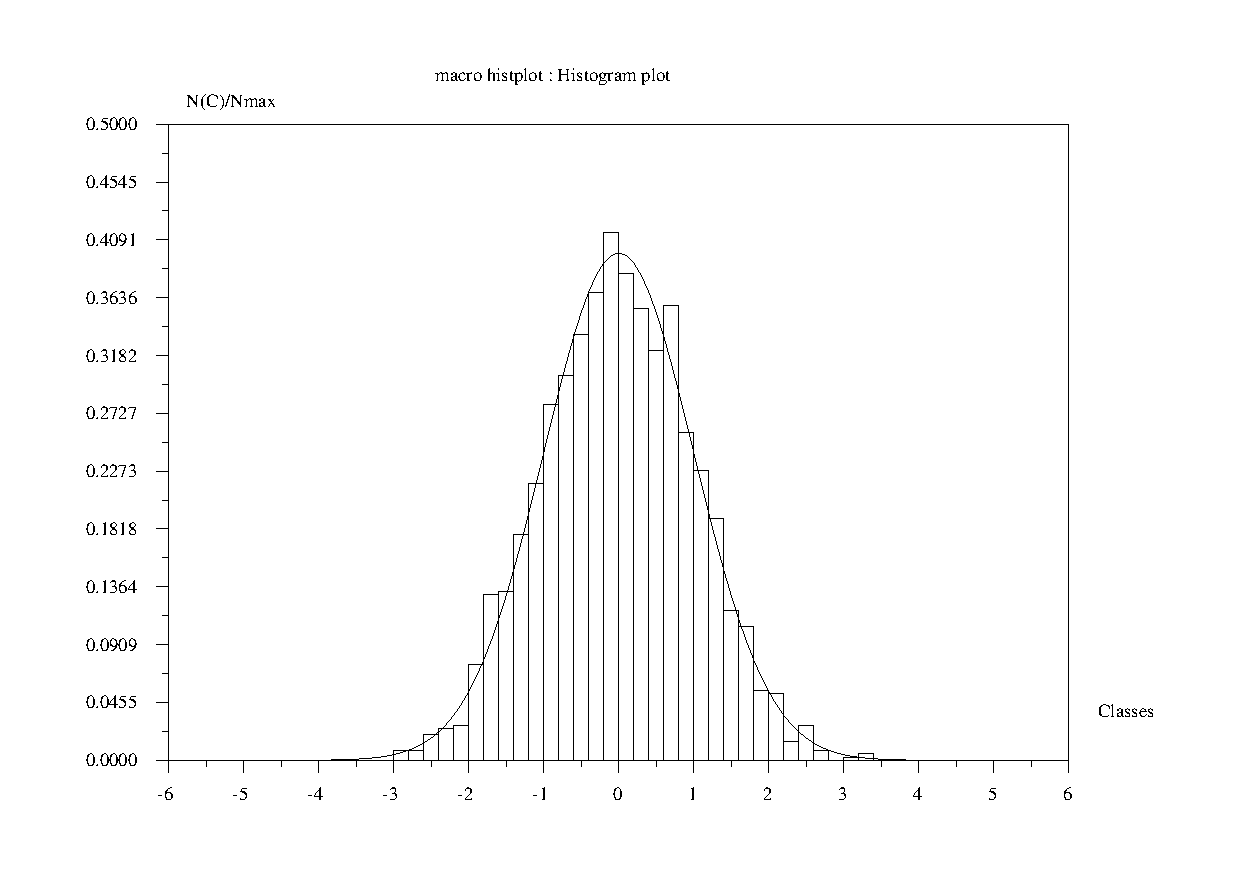
\includegraphics[width=.9\textwidth]{dummy-plot.eps}
    \caption{Esta es la figura sin caption}
    \label{fig:Hola}

  \let\@makecaption\oldcaption
  \makeatother
\end{figure}

\makeatletter
\newcommand\emptycaption[1]{%
  \let\oldcaption\@makecaption
  \long\def\@makecaption##1##2{\vskip \abovecaptionskip 
    \centering ##1
    \vskip\belowcaptionskip}
  \caption[#1]{#1}
  \let\@makecaption\oldcaption}
\makeatother

\begin{figure}[htbp]
  \centering
  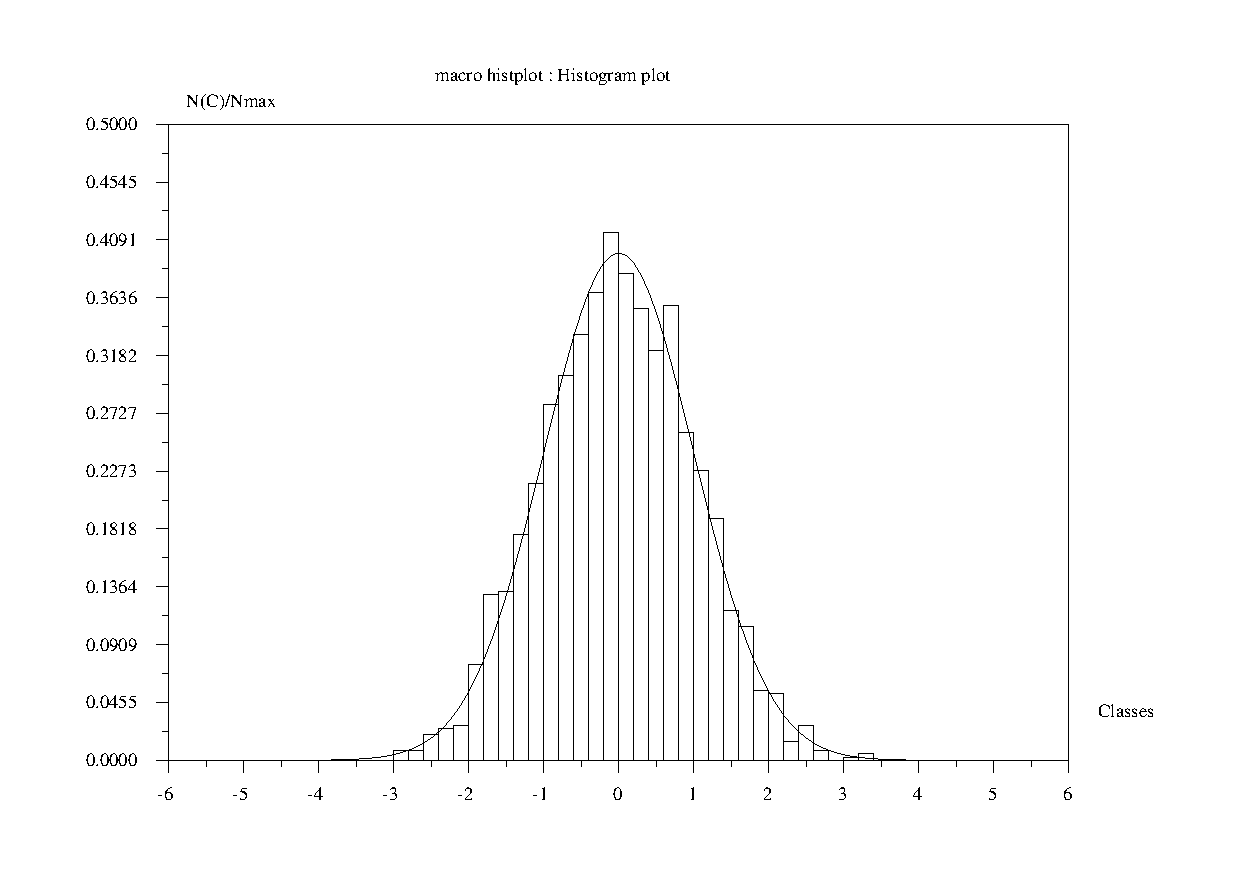
\includegraphics[width=.9\textwidth]{dummy-plot.eps}
  \emptycaption{Esta es la figura sin caption}
  \label{fig:Holabis}
\end{figure}

\begin{figure}[htbp]
  \centering
  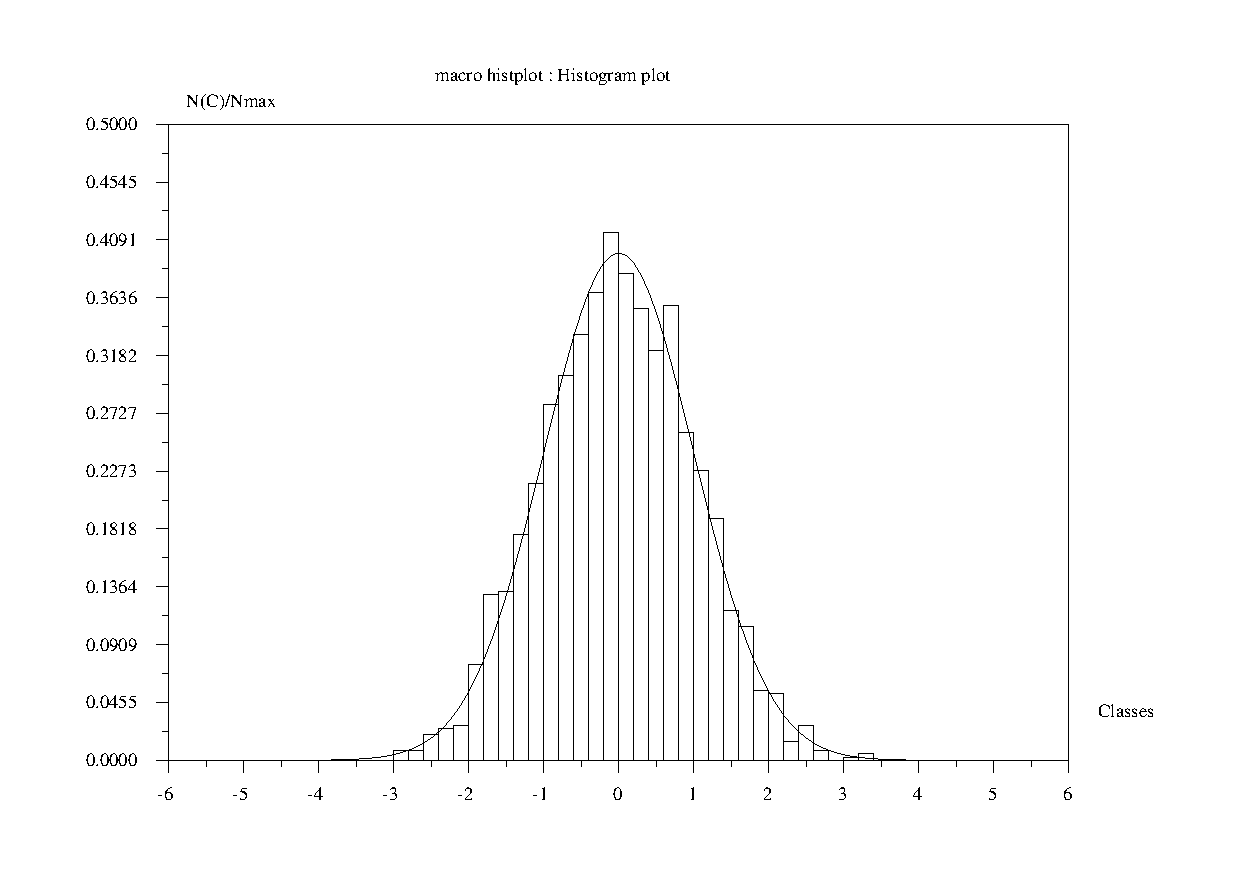
\includegraphics[width=.9\textwidth]{dummy-plot.eps}
  \caption{Esta es la figura CON caption}
  \label{fig:Hola2}
\end{figure}

\input{humpoutline.pstex_t}

\listoffigures

\end{document} 

%%% Local Variables: 
%%% mode: latex
%%% End: 
%%EOF
